%
% $RCSfile: data_mapper.tex,v $
%
% Copyright (c) 2004. Christian Heller. All rights reserved.
%
% No copying, altering, distribution or any other actions concerning this
% document, except after explicit permission by the author!
% At some later point in time, this document is planned to be put under
% the GNU FDL license. For now, _everything_ is _restricted_ by the author.
%
% http://www.cybop.net
% - Cybernetics Oriented Programming -
%
% http://www.resmedicinae.org
% - Information in Medicine -
%
% @author Christian Heller <christian.heller@tuxtax.de>
%

\paragraph{Data Mapper}
\label{data_mapper_heading}

Besides the \emph{Domain Logic}, standard three-tier architectures contain a
\emph{Data Source} layer which may for example represent a database. Both layers
need to exchange data. Modern systems use OOP methods to implement the domain
model. Database models, on the other hand, are often implemented as
\emph{Entity Relationship Model} (ERM).

In order to avoid close coupling and a mix-up of both layers, the introduction
of an additional \emph{Data Mapper} layer \cite{fowler2002} in between the two
others may be justified (figure \ref{datamapper_figure}). The most important
idea of this pattern is to abolish the interdependencies of domain- and
persistence model (database).

\begin{figure}[ht]
    \begin{center}
        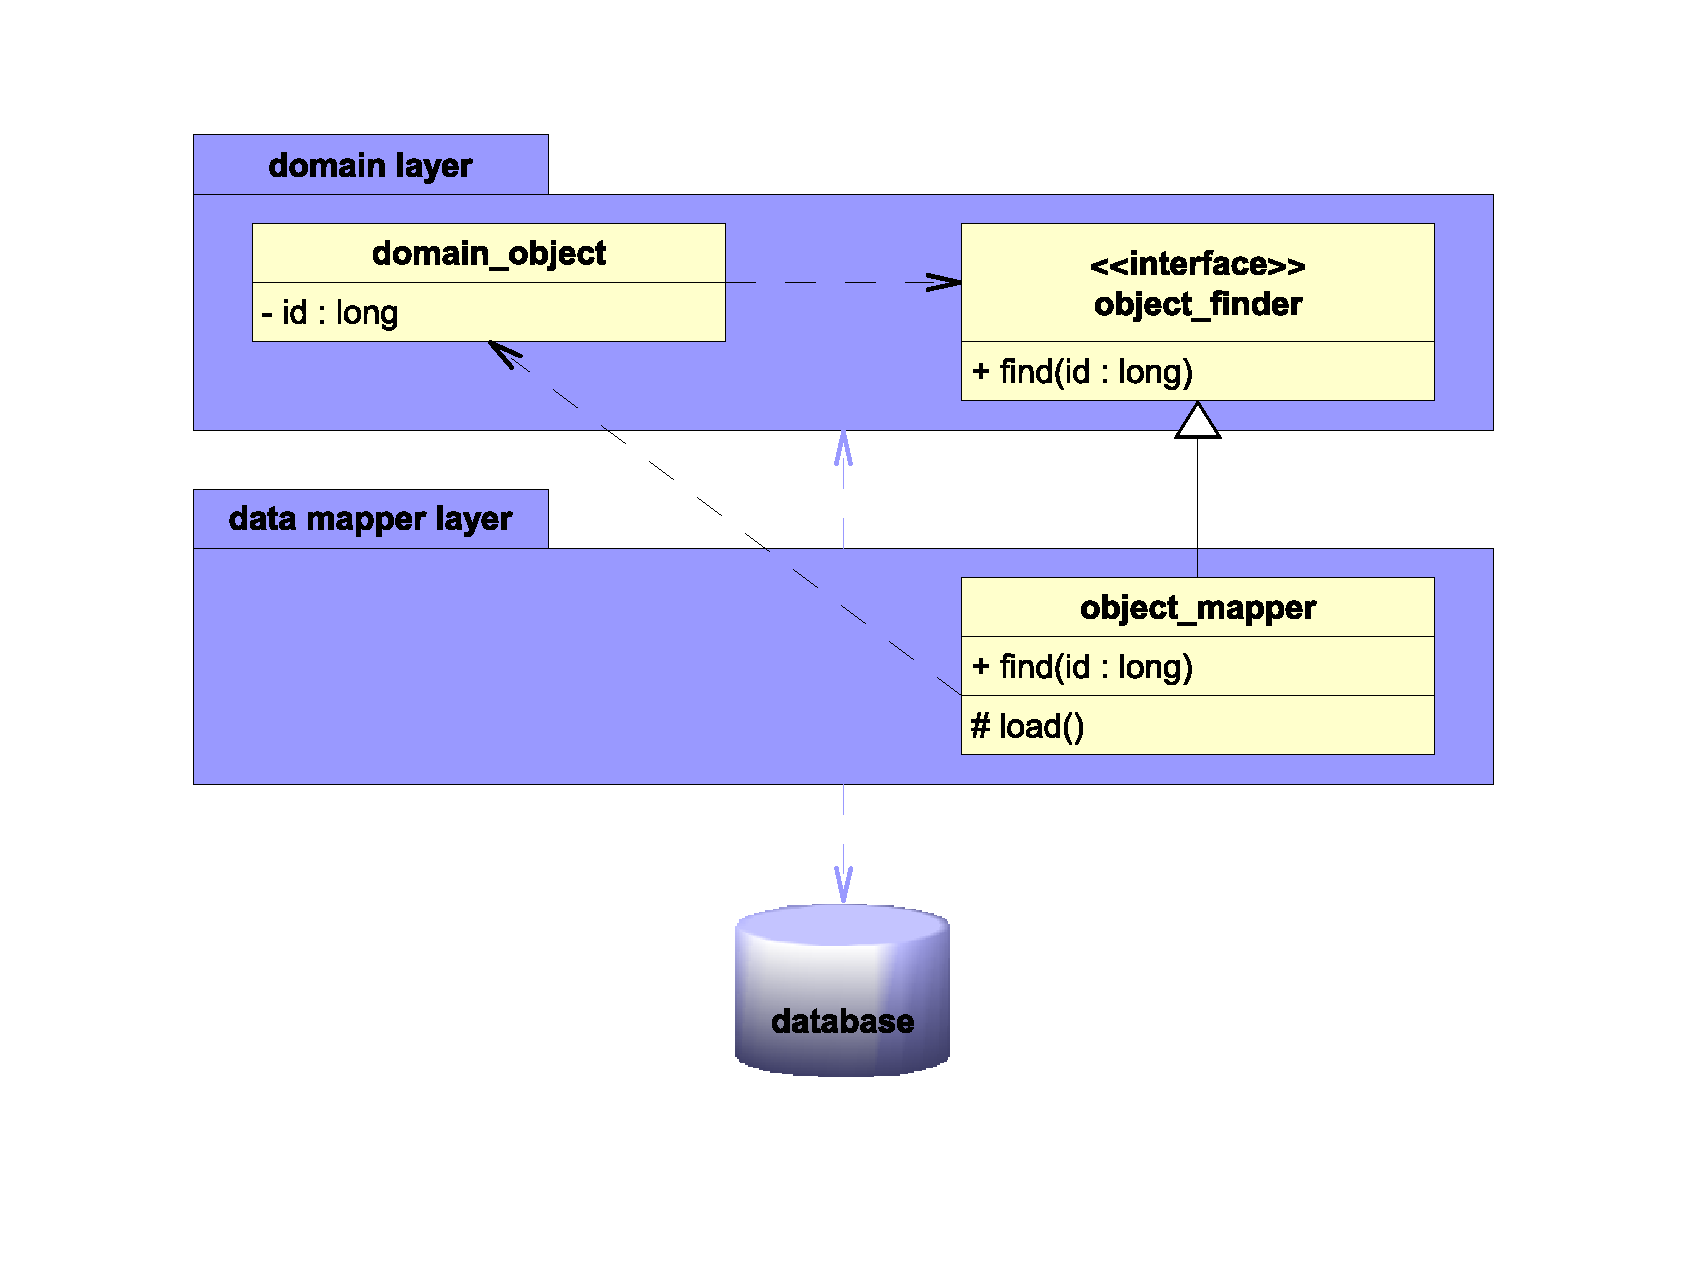
\includegraphics[scale=0.3]{vector/datamapper.eps}
        \caption{Data Mapper Pattern}
        \label{datamapper_figure}
    \end{center}
\end{figure}

The dashed arrows in figure \ref{datamapper_figure} indicate dependencies. The
data mapper layer knows the domain model- as well as the data source layer, via
\emph{unidirectional} relations. Its task is to \emph{translate} between the two,
in both directions. Domain model and data source know nothing from each other.

Each domain model class knows its appropriate interface (\emph{object\_finder})
but does not know the implementation of the same. That is, persistence- and
data retrieval mechanisms are hidden in front of the domain model. The
implementation (\emph{object\_mapper}) is part of the mapping package and also
implements all finder methods. It maps data of the received result sets to the
special attributes of the domain model objects.

The \emph{Mediator} pattern \cite{gamma1995} is similar to the \emph{Mapper}, in
that it is used to decouple different parts of a system. Fowler \cite{fowler2002}
writes: \textit{\ldots the objects that use a mediator are aware of it, even if
they aren't aware of each other; the objects that a mapper separates aren't even
aware of the mapper.}

Although the \emph{Data Mapper} pattern is very helpful at implementing OO
systems, two things are to be criticised:

Firstly, since the \emph{object\_finder} relies on functionality specific to the
retrieval of persistent data, it does actually belong into the data mapper layer
what, if done, would create bidirectional dependencies between the domain model-
and data mapper layer. But also with the \emph{object\_finder} remaining in the
domain model layer, dependencies are not purely unidirectional. It is true that
from an OO view, they are. Internally, however, a super class or interface
relates to its inheriting classes, so that it can call their methods to satisfy
the polymorphic behaviour.

Secondly, the layers do not truely build on each other. Taken a standard
architecture consisting of the following five -- instead of only three -- layers:

\begin{enumerate}
    \item Presentation
    \item Application Process
    \item Domain Model
    \item Data Mapper
    \item Data Source
\end{enumerate}

\ldots the application process does not only access the domain model layer, it
also has to manage (create and destroy) the objects of the data mapper layer.
In other words, it surpasses (disregards) the domain model layer when accessing
the data mapper layer directly.
